\documentclass{article}\usepackage[]{graphicx}\usepackage[]{color}
%% maxwidth is the original width if it is less than linewidth
%% otherwise use linewidth (to make sure the graphics do not exceed the margin)
\makeatletter
\def\maxwidth{ %
  \ifdim\Gin@nat@width>\linewidth
    \linewidth
  \else
    \Gin@nat@width
  \fi
}
\makeatother

\definecolor{fgcolor}{rgb}{0.345, 0.345, 0.345}
\newcommand{\hlnum}[1]{\textcolor[rgb]{0.686,0.059,0.569}{#1}}%
\newcommand{\hlstr}[1]{\textcolor[rgb]{0.192,0.494,0.8}{#1}}%
\newcommand{\hlcom}[1]{\textcolor[rgb]{0.678,0.584,0.686}{\textit{#1}}}%
\newcommand{\hlopt}[1]{\textcolor[rgb]{0,0,0}{#1}}%
\newcommand{\hlstd}[1]{\textcolor[rgb]{0.345,0.345,0.345}{#1}}%
\newcommand{\hlkwa}[1]{\textcolor[rgb]{0.161,0.373,0.58}{\textbf{#1}}}%
\newcommand{\hlkwb}[1]{\textcolor[rgb]{0.69,0.353,0.396}{#1}}%
\newcommand{\hlkwc}[1]{\textcolor[rgb]{0.333,0.667,0.333}{#1}}%
\newcommand{\hlkwd}[1]{\textcolor[rgb]{0.737,0.353,0.396}{\textbf{#1}}}%

\usepackage{framed}
\makeatletter
\newenvironment{kframe}{%
 \def\at@end@of@kframe{}%
 \ifinner\ifhmode%
  \def\at@end@of@kframe{\end{minipage}}%
  \begin{minipage}{\columnwidth}%
 \fi\fi%
 \def\FrameCommand##1{\hskip\@totalleftmargin \hskip-\fboxsep
 \colorbox{shadecolor}{##1}\hskip-\fboxsep
     % There is no \\@totalrightmargin, so:
     \hskip-\linewidth \hskip-\@totalleftmargin \hskip\columnwidth}%
 \MakeFramed {\advance\hsize-\width
   \@totalleftmargin\z@ \linewidth\hsize
   \@setminipage}}%
 {\par\unskip\endMakeFramed%
 \at@end@of@kframe}
\makeatother

\definecolor{shadecolor}{rgb}{.97, .97, .97}
\definecolor{messagecolor}{rgb}{0, 0, 0}
\definecolor{warningcolor}{rgb}{1, 0, 1}
\definecolor{errorcolor}{rgb}{1, 0, 0}
\newenvironment{knitrout}{}{} % an empty environment to be redefined in TeX

\usepackage{alltt}
\input{c:/aaaWork/zGnrlLatex/GnrlPreamble}
\hypersetup{pdftitle = R Workshop RStudio Getting Started}
\input{c:/aaaWork/zGnrlLatex/JustRPreamble}
\setcounter{secnumdepth}{0}  % have unnumbered sections appear in TOC
\IfFileExists{upquote.sty}{\usepackage{upquote}}{}
\begin{document}


\section{What is RStudio}
\vspace{-12pt}
R is an open-source software environment for statistical computing and graphics that runs on Windows, Mac OS, and many UNIX platforms.  Unlike many other programs, users interact with R through the issuance of commands on a command line rather than through a graphical user interface.    While such an interface may be unusual for many users, it's primary strength is the ability for a user to develop scripts of commands to perform various analyses that can then be easily repeated.

RStudio is an open-source integrated development environment (IDE) that serves as a front-end ``on top'' of R that eases the user's interaction with R by providing some of the conveniences of a GUI and, more importantly, a means for efficiently constructing and running R scripts.  Among other conveniences, RStudio provides a four-panel layout that includes a feature-rich source-code editor (includes syntax highlighting, parentheses completion, spell-checking, etc.), a tight link to the R console, a system for examining objects saved in R, an interface to R help, and extended features to examine and save plots.


\section{RStudio Design}
\vspace{-12pt}
RStudio is organized around a four-panel layout \figrefp{fig:RStudioLayout}.  The upper-left panel is the R \textit{Script Editor}.  R commands will be typed in this panel and submitted to the R \textit{Console} in the lower-left panel.  For most applications, you will be typing R commands in the \textit{Script Editor} and submitting them to the \textit{Console}; you will not be typing commands directly into the \textit{Console}.  The \textit{Script Editor} is a high-level text editor whereas the \textit{Console} is the R program.

\begin{figure}[h!]
  \centering
    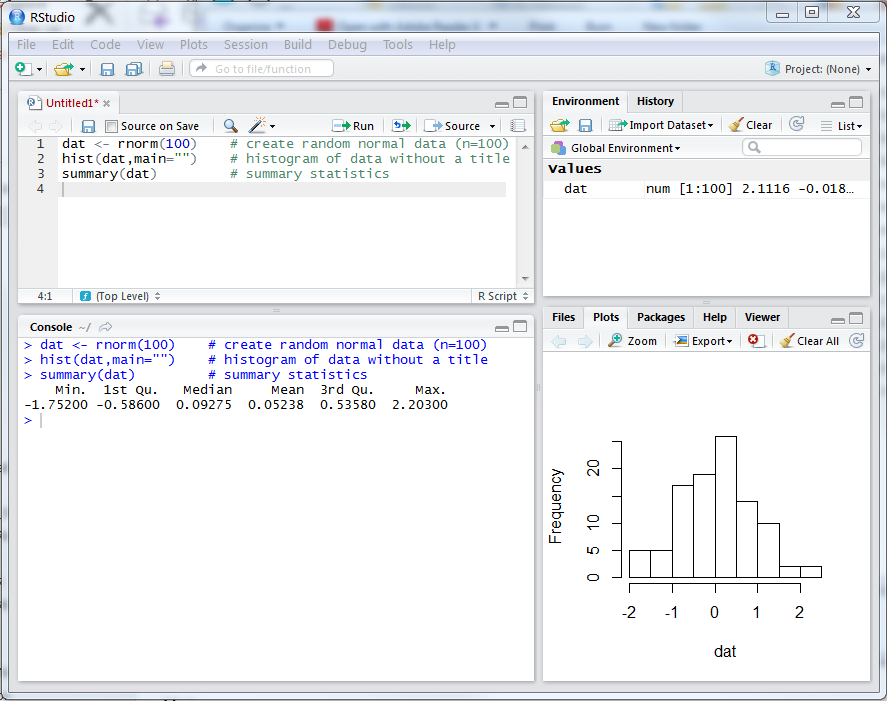
\includegraphics[width=6in]{Figs/RStudio_Intro_Layout.png}
    \caption{Example of the RStudio layout with the \textit{Script Editor} in the upper-left panel, \textit{Console} in the lower-left panel, the \textit{environment} tab shown in the upper-right panel, and the \textit{Plot} tab shown in the lower-right panel.}
  \label{fig:RStudioLayout}
\end{figure}

The upper-right panel contains at least two tabs -- \textit{Environment} and \textit{History}.  Many items listed under the \textit{Environment} tab can be double-clicked to open them for viewing as a tab in the \textit{Script Editor}.  The \textit{History} tab simply shows all of the commands that you have submitted to the \textit{Console} during the current session.

The lower-right panel contains five tabs -- \textit{Files}, \textit{Plots}, \textit{Packages}, \textit{Help}, and \textit{Viewer}.  The \textit{Plots} tab will show the high-level plots produced by commands submitted to the \textit{Console}.  One can cycle through the history of constructed plots with the arrows on the left side of the plot toolbar and plots can be saved to external files using the ``Export'' tab on the plot toolbar \figrefp{fig:RStudioLayout}.  A list of all installed packaged is seen by selecting the \textit{Packages} tab (packages can also be installed through this tab as described when you set-up RStudio).  Help for each package can be obtained by clicking on the name of package\footnote{Help can also be obtained by typing a question mark and then the name of the package in the console -- e.g., \R{?FSA}.}.  The help will then appear in the \textit{Help} tab.

\section{Basic Usage}
Our primary interaction with RStudio will be through developing R scripts in the \textit{Script Editor}, submitting those scripts to the \textit{Console}, and viewing textual or tabular results in the \textit{Console}, and graphical results in the \textit{Plot} panel.  In this section, I briefly introduce how to construct and run R scripts in RStudio.

One opens a blank file for an R script by selecting the ``New'' icon (
\includegraphics[scale=0.8]{Figs/RStudio_Icon_New.png}) and then \texttt{R Script}; selecting the \texttt{File} menu, \texttt{New} submenu, and \texttt{R Script} item; or with \verb+<CTRL>+ + \verb+<Shift>+ + \verb+N+.  In the ensuing tab of the \textit{Script Editor}, type the three lines exactly as shown below\footnote{For the moment, don't worry about what these lines ``do.''}.

\begin{knitrout}
\definecolor{shadecolor}{rgb}{0.969, 0.969, 0.969}\color{fgcolor}\begin{kframe}
\begin{alltt}
\hlstd{dat} \hlkwb{<-} \hlkwd{rnorm}\hlstd{(}\hlnum{100}\hlstd{)}    \hlcom{# create random normal data (n=100)}
\hlkwd{hist}\hlstd{(dat,}\hlkwc{main}\hlstd{=}\hlstr{""}\hlstd{)}    \hlcom{# histogram of data without a title}
\hlkwd{summary}\hlstd{(dat)}         \hlcom{# summary statistics}
\end{alltt}
\end{kframe}
\end{knitrout}

One must now ``submit'' these commands to the \textit{Console} to perform the requested calculations.  These commands can be submitted in a variety of ways:

\begin{itemize}
  \item Put the cursor on the first line in the \textit{Script Editor} and press the ``run'' icon (
\includegraphics[scale=0.8]{Figs/RStudio_Icon_Run.png}; altenatively press \verb+<CTRL>+ + \verb+<Enter>+).  This will submit the first line to the \textit{Console} and move the cursor to the second line in the \textit{Script Editor}.  Pressing the ``Run'' icon will now submit the second line.  And so on.
  \item Select all lines in the \textit{Script Editor} that you wish to submit and then press the ``run'' icon.
\end{itemize}

The RStudio layout after using the first method is shown in \figref{fig:RStudioLayout}.

The R Script in the \textit{Script Editor} should now be saved by selecting the \texttt{File} menu and the \texttt{Save} item (alternatively, pressing \verb+<CTRL>+ + \verb+S+).  RStudio can now be closed (do NOT save the workspace) and re-opened.  The script can then be re-opened (choose the \texttt{File} menu and the \texttt{Open file ...} submenu if the file is not already in the \textit{Script Editor}) and re-submitted to the \textit{Console} to exactly repeat the analyses\footnote{Note that the results of commands are not saved in R or RStudio; rather the commands are saved and re-submitted to re-perform the analysis.}.

\end{document}
